\documentclass[11pt]{article}
\usepackage[margin=2.5cm]{geometry}
\usepackage{amsmath,amssymb}
\usepackage{graphicx}
\usepackage{booktabs}
\usepackage{xcolor}
\usepackage{listings}
\usepackage[hidelinks]{hyperref}

\lstset{basicstyle=\ttfamily\small, columns=fullflexible, frame=single,
        framerule=0.3pt, rulecolor=\color{gray}, backgroundcolor=\color{gray!5},
        breaklines=true, showstringspaces=false}
\newcommand{\code}[1]{\texttt{#1}}
\newcommand{\chisq}{\chi^2}

\title{Notes on the GUNDAM fit for the ICARUS NuMI $\nu_e$CC inclusive analysis\\[4pt]
\large Dial interpolation, fit procedure, errors, and likelihood scans}
\author{}
\date{Draft, 6 October 2026}

\setlength{\emergencystretch}{2em}
\begin{document}
\maketitle
\tableofcontents

%======================================================================
\section{Scope and setup}
%======================================================================

These notes collect what was learned while debugging the GENIE morph knobs in the
fake-data studies, and explain how the GUNDAM fit works well enough to judge
whether a given fit can be trusted. Unless stated otherwise, everything refers to
\textbf{GUNDAM 1.9.X} as built in \code{GUNDAM-1.9.X/}, and to the configs in
\code{configsNue/}.

\begin{center}
\begin{tabular}{@{}ll@{}}
\toprule
Item & Setting \\
\midrule
Minimizer & Minuit2, Migrad (Simplex first), strategy 1, tolerance $10^{-2}$ \\
Errors & Hesse (\code{errors: "Hesse"}) \\
Fit space & normalized (\code{useNormalizedFitSpace: true}) \\
Likelihood & \code{PoissonLLH} \\
Parameter sets & template (true $E_e$ bins), GENIE, NuMI beamline, detector \\
Input MC & \code{gundam\_v30.root}, tree \code{events/NuMIFull/selected} \\
\bottomrule
\end{tabular}
\end{center}

The minimizer config is \code{Configs\_Minimizer/default\_minimizer.yaml}; the GENIE
parameter set is \code{Configs\_ParameterSet/GENIE/}.

%======================================================================
\section{How the GUNDAM fit is performed}
%======================================================================

\subsection{The model prediction}

Every MC event $e$ that passes the global and sample selection cuts carries a
nominal weight $w^{\rm nom}_e$, built from \code{nominalWeightFormula} (POT
scaling $\times$ \code{ppfx\_cv\_weight} for the neutrino MC). Each parameter
$\theta_k$ that applies to the event contributes a \emph{dial response}
$r_{ek}(\theta_k)$, so the event weight is
\begin{equation}
  w_e(\boldsymbol\theta) = w^{\rm nom}_e \prod_k r_{ek}(\theta_k).
\end{equation}
For the GENIE knobs, $r_{ek}$ is interpolated per event from the
\code{TClonesArray} of TGraphs stored in the input tree (Section~\ref{sec:dials}).
For the template parameters, $r_{ek} = \theta_k$ for events in true-$E_e$ bin $k$,
and 1 otherwise.

The predicted content of reconstructed bin $b$ is then
$\mu_b(\boldsymbol\theta) = \sum_{e\in b} w_e(\boldsymbol\theta)$, and $d_b$ is the
(fake) data in the same bin.

Per-dataset selection is possible: each \code{mc} and \code{data} block in a
dataset accepts \code{selectionCutFormula} (a string, or a list joined with
\code{\&\&}), applied before the per-sample cuts.

\subsection{The likelihood}

GUNDAM minimizes a quantity on the $-2\ln L$ (i.e.\ $\chisq$-like) scale:
\begin{equation}
  \mathcal{L}(\boldsymbol\theta) \equiv \text{llh}
  = \underbrace{\sum_b 2\left[\mu_b - d_b + d_b\ln\frac{d_b}{\mu_b}\right]}_{\text{llhStat}}
  \;+\; \underbrace{\sum_{\text{sets}} \boldsymbol\Delta^{T} V^{-1} \boldsymbol\Delta}_{\text{llhPenalty}},
  \qquad \boldsymbol\Delta = \boldsymbol\theta - \boldsymbol\theta^{\rm prior}.
  \label{eq:llh}
\end{equation}
The stat term is the Baker--Cousins Poisson form
(\code{PoissonLogLikelihood.h}); bins with $d_b=0$ contribute $2\mu_b$, and a
bin with $\mu_b\le 0$ gives $+\infty$. The penalty term is computed per parameter
set from its prior covariance $V$ (\code{LikelihoodInterface.cpp}); a set with no
covariance matrix, such as the template parameters, contributes nothing and is
constrained only by the data.

Because \code{llh} is on the $-2\ln L$ scale, Minuit's default
\code{ErrorDef} $=1$ is the correct one: $\Delta\text{llh} = 1$ defines the
$1\sigma$ interval for a single parameter.

\subsection{Minimization}

\begin{enumerate}
  \item \textbf{Normalized fit space.} With \code{useNormalizedFitSpace: true}
    the minimizer sees $\tilde\theta_k = (\theta_k - \theta^{\rm prior}_k)/\sigma_k$,
    so every parameter has prior 0 and width 1. Covariances are converted back
    afterwards by multiplying by $\sigma_i\sigma_j$
    (\code{RootMinimizer.cpp}).
  \item \textbf{Simplex} runs first with a loose tolerance to get near the
    minimum.
  \item \textbf{Migrad} then descends using the gradient and an iteratively
    built approximation to the Hessian, stopping when the estimated distance to
    the minimum (EDM) is below $0.002 \times \text{tolerance}$ (Minuit2 convention,
    $\text{UP}=1$).
  \item \textbf{Hesse} recomputes the full matrix of second derivatives at the
    minimum by finite differences and inverts it to get the post-fit covariance
    (Section~\ref{sec:errors}).
\end{enumerate}

Parameters with bounds (\code{parameterLimits}, or the lower/upper-bound vectors
in a covariance file) are handled by Minuit through a sine transform to an
unbounded internal variable. This matters for errors near a bound
(Section~\ref{sec:bounds}).

The post-fit values are written to \code{FitterEngine/postFit/parState\_TNamed}
and the covariance to \code{FitterEngine/postFit/Hesse/hessian/}; the toy
generator and \code{gundamCalcXsec} read these back.

%======================================================================
\section{GENIE dials: splines, graphs and morph knobs}
\label{sec:dials}
%======================================================================

\subsection{Two kinds of GENIE knob}

\begin{description}
  \item[Multisigma knobs] (e.g.\ \code{MaCCRES}, \code{NormCCMEC}) scale a model
    parameter by some number of standard deviations. The response is meaningful
    for both signs, and $\theta=\pm1$ is a genuine $\pm1\sigma$ variation.
  \item[Morph knobs] (\code{VecFFCCQEshape}, \code{DecayAngMEC},
    \code{Theta\_Delta2Npi}, \code{ThetaDelta2NRad}) interpolate between two
    models: $\theta=0$ is the GENIE nominal and $\theta=1$ is the alternative
    model. Negative values have no model behind them.
\end{description}

In the covariance file built by
\code{GENIE/makeParameterRootFile.C}, both kinds get prior 0, $\sigma=1$, and no
correlations (only the four Z-expansion knobs are correlated). The one
exception is a prior of 0.005 on \code{VecFFCCQEshape}, which appears to be a
workaround for the zero-slope problem described below.

\subsection{What is actually stored}

Inspecting the first 11{,}729 events of \code{gundam\_v30.root} shows that all four
morph knobs are stored at $x = \{-1,-0.5,0,0.5,1\}$ and are \textbf{exactly
symmetric}, $w(-x)=w(x)$, in every event with a non-trivial response:

\begin{center}
\begin{tabular}{@{}lrl@{}}
\toprule
Knob & Non-flat events & Example $w(x)$ at $x=-1,\dots,1$ \\
\midrule
\code{Theta\_Delta2Npi} & 2798 & 1.179, 1.090, 1.000, 1.090, 1.179 \\
\code{ThetaDelta2NRad}  & 24   & 0.197, 0.598, 1.000, 0.598, 0.197 \\
\code{DecayAngMEC}      & 1367 & 0.066, 0.533, 1.000, 0.533, 0.066 \\
\code{VecFFCCQEshape}   & 4655 & 1.027, 1.014, 1.000, 1.014, 1.027 \\
\bottomrule
\end{tabular}
\end{center}

So the upstream weight production has already mirrored the morph knobs. The
physical information lives entirely on $x\in[0,1]$.

\subsection{Spline vs Graph dials}

GUNDAM builds each event's response from those knots according to
\code{dialType}:

\begin{description}
  \item[\code{Spline}] A cubic spline through all knots. The default subtype is
    ``not-a-knot'' (same curve as ROOT's \code{TSpline3}); \code{dialSubType}
    can select \code{natural}, \code{catmull-rom}, or \code{monotonic}.
  \item[\code{Graph}] Linear interpolation between neighbouring knots.
\end{description}

\begin{figure}[h]
  \centering
  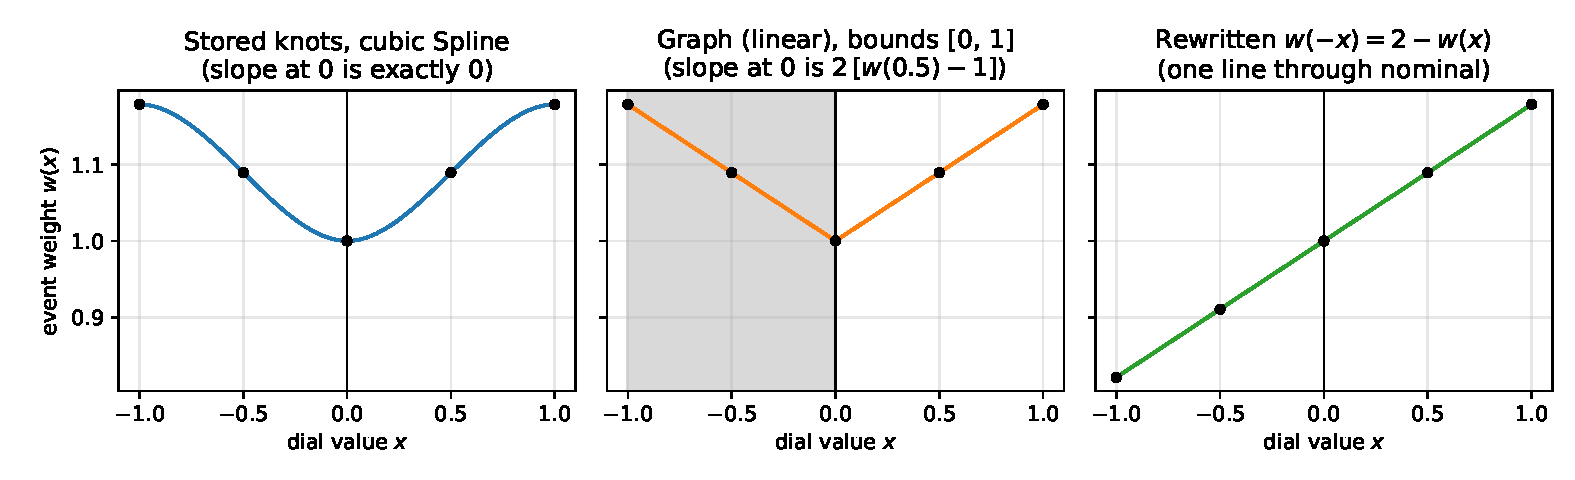
\includegraphics[width=\textwidth]{fig_morph_dials.pdf}
  \caption{One \code{Theta\_Delta2Npi} event from \code{gundam\_v30.root}.
    Left: the default cubic spline through the symmetric knots has zero slope
    at the nominal point. Middle: a linear Graph dial restricted to $[0,1]$
    (grey region excluded by the bounds). Right: the knots rewritten as
    $w(-x)=2-w(x)$, giving one straight line through nominal.}
  \label{fig:dials}
\end{figure}

For a symmetric set of knots, \textbf{any} smooth spline has zero slope at
$x=0$ (Fig.~\ref{fig:dials}, left). The prediction $\mu_b$ is then flat to first
order around nominal for every event, so:
\begin{itemize}
  \item $\partial\mathcal{L}/\partial\theta = 0$ at $\theta=0$ regardless of the
    data, so the nominal point is always a stationary point and Migrad has no
    gradient to follow;
  \item the data enters the curvature only through the
    $(1-d_b/\mu_b)\,\partial^2\mu_b$ term of Eq.~\eqref{eq:hess}, which can be
    negative and can cancel the prior (Section~\ref{sec:errors}).
\end{itemize}
This is what produced the post-fit \code{Theta\_Delta2Npi} $= 0.00 \pm 3.7$ in the
\code{emb} fake-data study.

\subsection{Mirroring}

GUNDAM's \code{useMirrorDial} with \code{mirrorLowEdge}/\code{mirrorHighEdge}
folds the fit parameter back into the given range before the dial is evaluated
(\code{DialInputBuffer.cpp}): a value past an edge reflects back, so with edges
$\pm1$ a value of 1.5 is evaluated at 0.5 and 3.0 at $-1$. This only prevents
extrapolation beyond the knots. Because the stored response is already
symmetric, mirroring at $[-1,1]$ or at $[0,1]$ changes nothing, which is why
setting \code{mirrorLowEdge: 0} had no effect.

\subsection{Options and recommendation}

\begin{enumerate}
  \item \textbf{Graph dial, bounds $[0,1]$, no mirroring} (current choice).
    Linear interpolation on $[0,1]$ has slope $2[w(0.5)-1]\neq0$ at nominal, so the
    data supplies a gradient and the double minimum at $\pm\theta$ is removed.
    Costs: a kink in slope at the 0.5 knot, and nominal sits on the lower
    bound, so errors for a fit that ends near 0 are one-sided.
  \item \textbf{Rewrite the negative knots as $w(-x)=2-w(x)$} in the input tree,
    then use Graph or Spline with bounds of about $[-3,3]$. One straight line
    through nominal: no zero slope, no bound at nominal, normal Gaussian prior
    and Hesse behaviour. Negative values are a linear extrapolation with no
    model behind them; large negative pulls should be read as tension, not
    physics. Weights can go negative where $w(1)$ is large (e.g.\
    \code{DecayAngMEC}); \code{minimumSplineResponse: 0} clamps them to 0,
    re-introducing a kink.
\end{enumerate}
Mirroring ($w(-x)=w(x)$) is worse than either because it gives zero slope at
nominal, a $\pm\theta$ degeneracy that a Gaussian prior at 0 cannot describe, and
no way for the data to pull the knob ``away from'' the alternative model.

All four morph knobs should be treated the same way, even those that look well
behaved in a particular fit: the zero slope is a property of the stored
splines, not of the data. With the Graph dial, the 0.005 prior on
\code{VecFFCCQEshape} is no longer needed.

\paragraph{Housekeeping.} \code{CC1piTPi} and \code{LowQ2Suppression} are in
\code{knoblist.py} and \code{GENIEDialsDef.yaml} but not in the knob lists of
\code{makeParameterRootFile.C}; check that \code{gundaminput\_geniesyst.root}
actually contains priors for them.

Example dial definition:
\begin{lstlisting}
- parameterName: "Theta_Delta2Npi"
  isEnabled: true
  dialSetDefinitions:
    - dialType: Graph
      minimumSplineResponse: 0
      applyOnDataSets: ["ICARUSNuMI_nueCCInclusive"]
      dialLeafName: "Theta_Delta2Npi"
      applyCondition: "[reco_is_data]==0"
\end{lstlisting}

%======================================================================
\section{Errors and the Hessian}
\label{sec:errors}
%======================================================================

\subsection{From curvature to covariance}

Near the minimum $\hat{\boldsymbol\theta}$ the likelihood is approximated by a
quadratic,
\begin{equation}
  \mathcal{L}(\boldsymbol\theta) \approx \mathcal{L}(\hat{\boldsymbol\theta})
  + \tfrac12 (\boldsymbol\theta-\hat{\boldsymbol\theta})^{T} H
    (\boldsymbol\theta-\hat{\boldsymbol\theta}),
  \qquad H_{ij} = \frac{\partial^2\mathcal{L}}{\partial\theta_i\partial\theta_j}.
\end{equation}
Since $\mathcal{L}$ is $-2\ln L$, the covariance is
\begin{equation}
  C = 2\,H^{-1},
\end{equation}
and $\sigma_i = \sqrt{C_{ii}}$ is the Hesse error. For a single uncorrelated
parameter this is the half-width at which $\mathcal{L}$ rises by 1.

\subsection{What contributes to the curvature}

Differentiating Eq.~\eqref{eq:llh} twice for one parameter $\theta$:
\begin{equation}
  \frac{\partial^2\mathcal{L}}{\partial\theta^2}
  = \underbrace{\frac{2}{\sigma_{\rm prior}^2}}_{\text{penalty}}
  \;+\; 2\sum_b \Bigg[
      \underbrace{\frac{d_b}{\mu_b^2}\Big(\frac{\partial\mu_b}{\partial\theta}\Big)^2}_{\ge 0}
      \;+\;
      \underbrace{\Big(1-\frac{d_b}{\mu_b}\Big)\frac{\partial^2\mu_b}{\partial\theta^2}}_{\text{either sign}}
  \Bigg].
  \label{eq:hess}
\end{equation}
Consequences:
\begin{itemize}
  \item The first data term is never negative, so a dial with a real slope can
    only \emph{tighten} the error below the prior.
  \item For an Asimov fit, $d_b=\mu_b$ at the minimum and the second data term
    vanishes; the post-fit error is then always $\le$ the prior.
  \item A post-fit error \textbf{larger than the prior} is only possible when the
    second term is negative, i.e.\ the response is curved, the data disagrees
    with the prediction, and the slope is small. For \code{Theta\_Delta2Npi},
    $1/3.7^2 \approx 0.07$, so the data term cancelled about 93\% of the prior
    curvature. That is a diagnostic, not a real $3.7\sigma$ uncertainty.
\end{itemize}

\subsection{Marginal vs conditional errors}

$\sqrt{C_{ii}}$ is the \emph{marginal} error: it allows all other parameters to
move. The \emph{conditional} error, with all others fixed at the best fit, is
$1/\sqrt{(C^{-1})_{ii}} \le \sqrt{C_{ii}}$. They agree only when $\theta_i$ is
uncorrelated with everything else. One-dimensional scans
(Section~\ref{sec:scans}) measure the conditional width.

\subsection{When the Hesse error can be trusted}
\label{sec:bounds}

These are conditions for the symmetric Hesse error to be a valid
\emph{summary} of a parameter. Failing them does not mean the fit is bad; it
means the parameter needs a different summary. The Hesse error assumes
$\mathcal{L}$ is a parabola out to $\pm1\sigma$. Check:
\begin{enumerate}
  \item \textbf{Interval inside the bounds.} At a bound the sine transform has
    zero derivative and the external error is unreliable. More generally, if
    $\hat\theta\pm\sigma$ crosses a bound, the true interval is one-sided. For
    bounded parameters such as the morph knobs this is expected, not a failure;
    see Section~\ref{sec:bounded}.
  \item \textbf{Not at a kink.} A Graph dial has a slope discontinuity at each
    knot (0.5 for the morph knobs); finite differences across it give a
    curvature that depends on which side is sampled.
  \item \textbf{Smooth and parabolic over $\pm1\sigma$.} Asymmetric or flat
    regions mean the quadratic approximation fails.
\end{enumerate}
If any check fails, use a likelihood scan or MINOS (\code{errors: "Minos"}) and
read the interval where $\Delta\mathcal{L}=1$, clipped at the bounds.

\subsection{Bounded parameters: the morph knobs on $[0,1]$}
\label{sec:bounded}

With a Graph dial and bounds $[0,1]$, a morph knob is a different statistical
object from a multisigma knob, and the Gaussian-error language above does not
apply to it directly.

\paragraph{What the prior is.} The Graph is the dial \emph{response}; the prior
is the penalty term $\theta^2/\sigma^2$ with prior 0 and $\sigma=1$. Truncated by
the bounds, it is a half-Gaussian on $[0,1]$: staying at the nominal model costs
nothing, and switching fully to the alternative model costs
$\Delta\text{llh}=1$. This encodes the usual convention that the alternative
model is a ``$1\sigma$'' variation. A different belief needs a different prior:
for example, if both models are considered equally plausible, a flat prior on
$[0,1]$ (no penalty) is more appropriate.

\paragraph{The prior width already spans the whole range.} Since $\sigma=1$
equals the width of the allowed range, $\hat\theta\pm\sigma$ will cross a bound
for any morph knob the data does not strongly constrain. That is a consequence
of the parametrization, not a symptom of a bad fit.

\paragraph{Sitting at a bound can be the right answer.} $\hat\theta=0$ means the
data prefers the nominal model; $\hat\theta=1$ means it prefers the full
alternative. Both are physically sensible outcomes for an on/off effect. What
to check instead:
\begin{itemize}
  \item In a scan, \code{llh} should \emph{rise} moving away from the bound into
    the allowed region. If it falls, the minimizer stopped early.
  \item Report a one-sided interval from the scan, e.g.\ $\theta < \theta_{1}$ where
    $\Delta\text{llh}(\theta_{1}) = 1$ relative to the value at the bound, rather
    than the Hesse $\pm$ error.
  \item For an interior best fit, read the two crossings of $\Delta\text{llh}=1$
    separately, clipped at 0 and 1; they will generally be asymmetric.
\end{itemize}

\paragraph{Where it does matter: throws.} The toy generator and
\code{gundamCalcXsec} throw parameters from the post-fit (Hesse) covariance as a
multivariate Gaussian. In GUNDAM~1.9 a throw that puts any parameter outside its
bounds is rejected and the whole vector re-thrown
(\code{ParametersManager.cpp}), so morph knobs are sampled from a truncated
Gaussian whose width comes from the Hesse matrix. Two consequences:
\begin{itemize}
  \item If the Hesse width is unreliable (best fit at or near a bound), the
    throws inherit that error. Compare the spread of thrown morph values with
    the scan.
  \item The acceptance is low: a knob at 0 with width 1 lands in $[0,1]$ about
    34\% of the time, so four such knobs accept roughly 1\% of throws.
\end{itemize}
If this becomes a problem, rewriting the knots as $w(-x)=2-w(x)$ and removing
the bounds (Section~\ref{sec:dials}) makes the morph knobs ordinary Gaussian
parameters, for which Hesse and Gaussian throws are both valid. That is the
main practical argument for that option.

%======================================================================
\section{Likelihood scans}
\label{sec:scans}
%======================================================================

\subsection{What the scan produces}

With \code{enablePostFitScan: true} (and/or \code{enablePreFitScan}) in
\code{fitterEngineConfig}, GUNDAM steps each free fit parameter across a range
around its current value, holding all others fixed, and records at each point:

\begin{description}
  \item[\code{llhPenalty}] the prior term of Eq.~\eqref{eq:llh}. Independent of the
    data. For an uncorrelated knob it is the parabola $(\theta-\theta^{\rm prior})^2/\sigma^2$;
    for correlated knobs its minimum can be shifted; for the template
    parameters it is flat at 0.
  \item[\code{llhStat}] the Poisson data term. Shows what the data alone says
    about the knob.
  \item[\code{llh}] the sum, i.e.\ what the fit minimizes.
\end{description}
Optional extras (\code{llhStatPerSample}, per-bin and per-sample weight scans)
are enabled in \code{scanConfig}.

\paragraph{GUNDAM 1.9 bug.} With the post-fit scan enabled, 1.9 crashed with
\code{TDirectoryFile::mkdir: An object with name
Template\_Parameter\_true\_leading\_electron\_energy exists already}, followed by a
segfault. The scanner writes \code{<full title>\_CurrentPar}, whose name contains
a \code{/}; the write helper turns it into an unchecked \code{mkdir}, which fails
on the second parameter of a set and returns a null directory. Fixed locally in
\code{ParameterScanner.cpp} by replacing \code{/} with \code{\_} in that name, as is
already done for the scan graphs. Requires a rebuild of 1.9.

\subsection{Reading the shapes}

\begin{figure}[h]
  \centering
  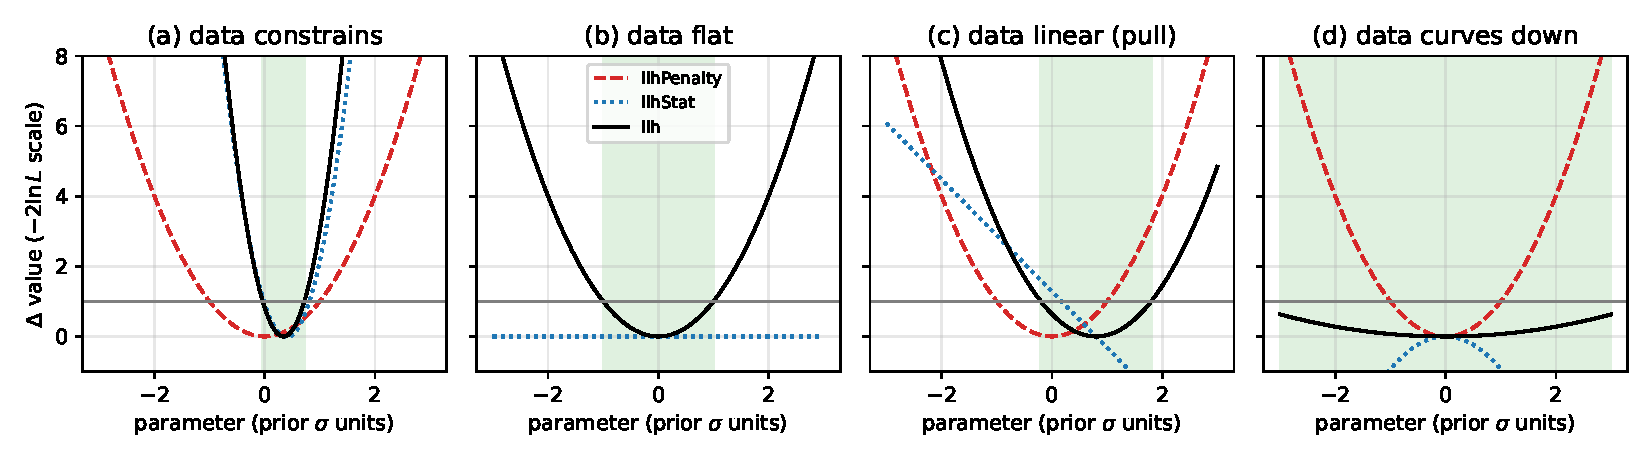
\includegraphics[width=\textwidth]{fig_scan_shapes.pdf}
  \caption{Illustrative scan shapes (toy curves, not from a fit), in units of the
    prior $\sigma$ with prior at 0. The shaded band is where
    $\Delta\text{llh}\le1$. (a) Data constrains the knob: narrow total, error well
    below 1. (b) Data flat: total equals the prior, error $\approx 1$. (c) Data
    linear: total is the prior parabola shifted by half the slope; error still
    $\approx 1$. (d) Data curves downward: total is much flatter than the prior,
    error $\gg 1$, as for \code{Theta\_Delta2Npi} with the original spline.}
  \label{fig:scans}
\end{figure}

\begin{center}
\begin{tabular}{@{}p{0.32\textwidth}p{0.6\textwidth}@{}}
\toprule
llhStat shape & Interpretation \\
\midrule
Deep, narrow valley & Data constrains the knob; post-fit error well below prior. \\
Flat & Knob does not change the selected-sample prediction; error $\approx$ prior. \\
Linear & Data pulls one way with no curvature; best fit shifts by about
  half the slope (in $\chisq$ per $\sigma$), error $\approx$ prior. \\
Curving downward & Data term reduces the curvature; error larger than prior.
  Check the dial shape and whether the fit sits at a stationary point. \\
Minimum far from prior & Data and prior disagree. In a fake-data study, often the
  knob absorbing the injected variation; otherwise, a mismodelling to understand. \\
Kinks, steps, jagged & Dial problem: interpolation knots, weights clamped by
  \code{minimumSplineResponse}, or bad splines. \\
\bottomrule
\end{tabular}
\end{center}

\subsection{Using scans to decide whether the fit succeeded}

\begin{enumerate}
  \item \textbf{Minimum at the centre.} Post-fit scans are centred on the best fit,
    so \code{llh} should have its minimum there. A minimum elsewhere means the
    minimizer did not converge in that direction.
  \item \textbf{Width matches Hesse.} Read where \code{llh} rises by 1 on each side.
    If it is close to $\pm\sigma_{\rm Hesse}$ and parabolic, the Hesse error is
    fine. If it is asymmetric, kinked, or hits a bound first, quote the scan
    interval instead. A scan narrower than Hesse is expected for correlated knobs
    (conditional vs marginal); check the post-fit correlation matrix.
  \item \textbf{What sets the error.} Compare the steepness of \code{llhStat} and
    \code{llhPenalty}. Data-dominated knobs should have post-fit errors well below
    1; prior-dominated knobs about 1; anything above 1 needs explaining.
  \item \textbf{Physical behaviour.} Smooth curves indicate healthy dials; kinks or
    steps point at the dial definition or input splines.
\end{enumerate}

\subsection{Unconstrained systematics are not bad systematics}

A flat or linear \code{llhStat} means the fit cannot reduce that uncertainty, so
its full prior propagates into the result. That is correct behaviour. Such knobs
must be kept: they often act through the efficiency and background subtraction
in the extracted cross section, which the selected sample may not be sensitive
to. Dropping a knob is only justified if it has no effect on anything reported:
check the $\pm1\sigma$ event-rate variations (\code{preFit/oneSigma},
\code{preFit/varyEventRates}) and the change in the \code{gundamCalcXsec} throw
spread when the knob is fixed.

%======================================================================
\section{Why the extracted cross-section uncertainty is large}
\label{sec:xsecunc}
%======================================================================

The post-fit \emph{distribution} (reconstructed event rate) carries a small
uncertainty, a few percent per bin, while the extracted \emph{cross section} in
true-$E_e$ bins is $20$--$32\%$. Both come from the same fit and the same
post-fit covariance. This section explains the gap, using a breakdown study
driven by \code{run\_frac\_uncertainty.sh}, which re-runs the fit,
\code{gundamCalcXsec}, and the toy generator with individual systematic groups
switched on or off (variants \code{template\_only}, \code{xsec\_only},
\code{flux\_only}, \code{detector\_only}, \code{all}, and the N$-$1 variants
\code{no\_xsec}/\code{no\_flux}/\code{no\_detector}). All numbers below are
Asimov, at $2.5\times10^{20}$ POT.

\subsection{The flux--template degeneracy}

The predicted events in true bin $i$ factorize as
\begin{equation}
  N_i \;=\; \Phi \cdot \sigma_i \cdot \epsilon_i \cdot T \cdot (\dots),
  \label{eq:Nfact}
\end{equation}
with flux $\Phi$, cross section $\sigma_i$, efficiency $\epsilon_i$, and number
of targets $T$. The template parameters $t_i$ are \emph{free} (no prior
covariance; bounds $[0,3]$ only), one per true-$E_e$ bin, and multiply
$\sigma_i$. Every factor in Eq.~\eqref{eq:Nfact} enters multiplicatively, so a
shift in $\Phi$, $\epsilon_i$, or any reweighting systematic produces the same
change in $N_i$ as a change in $t_i$. With ten free templates spanning all
per-bin rescalings, any systematic whose effect is a rescaling of the
true-$E_e$ spectrum is reproduced exactly by the templates.

The fit therefore constrains only the \emph{product} $t_i\times(\text{syst})$,
which the data pins down, not the split. Along the degenerate direction the data
term of Eq.~\eqref{eq:llh} is flat; the tie-break is the penalty. A systematic
has a Gaussian prior ($\sigma=1$) and stays at it; the template has no prior and
absorbs the shift, its post-fit error inflating. ``The template absorbs the
systematic'' and ``the systematic stays at its prior'' are the same statement.
This extends Section~\ref{sec:scans} (``Unconstrained systematics are not bad
systematics'') to the normalization of the signal itself.

\paragraph{A mechanical picture.} (Figs.~\ref{fig:balance} and~\ref{fig:spring})
Think of each parameter as a bead the fit displaces from nominal. The prior attaches a spring of stiffness
$2/\sigma_{\rm prior}^2$ (the penalty term of Eq.~\eqref{eq:hess}); the data
attaches a second spring whose stiffness is the first data term,
$2\sum_b (d_b/\mu_b^2)(\partial\mu_b/\partial\theta)^2$, and therefore grows with
the event counts $d_b$. The template parameters carry \emph{no} prior spring.
Pushed along a degenerate direction, the free templates---restrained by
nothing---slide all the way to absorb it, while a systematic, held by its prior
spring, barely moves. Low event counts make the data spring weak, so even a
systematic with some distinguishing power stays pinned near its prior: this is
why, at this sample size, the systematics scarcely move and the templates take
up essentially all of the variation. More statistics stiffens the data spring,
but only along the directions the response matrix makes distinguishable
(the diagonal test below); along an exactly degenerate direction the data spring
has zero stiffness no matter the counts, which is the $\sigma=1.000$ limit.

\begin{figure}[h]
  \centering
  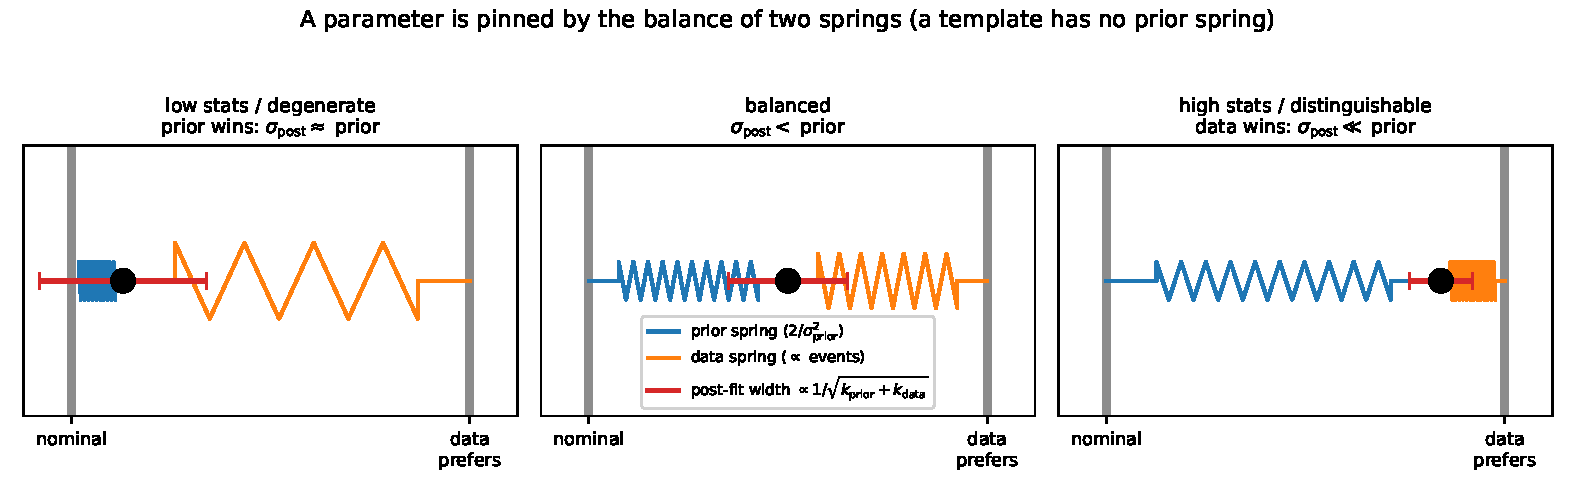
\includegraphics[width=\textwidth]{fig_xsec_balance.pdf}
  \caption{How well a single parameter is pinned is the balance of two springs
    (Eq.~\eqref{eq:hess}): a prior spring of stiffness $2/\sigma_{\rm prior}^2$
    tying it to nominal, and a data spring whose stiffness grows with the event
    count, pulling it toward the data-preferred value. The post-fit width is
    $\propto 1/\sqrt{k_{\rm prior}+k_{\rm data}}$ (red bar). Left: with few events,
    or along a degenerate direction, the data spring is limp, the prior wins, and
    the parameter stays near nominal with $\sigma_{\rm post}\approx$ prior. Right:
    with many events and a distinguishable response the data spring is stiff and
    the parameter is pulled to the data value and tightly constrained. A template
    parameter has no prior spring at all (left anchor removed); it is held only by
    the data spring, and in an exactly degenerate direction by nothing.}
  \label{fig:balance}
\end{figure}

\begin{figure}[h]
  \centering
  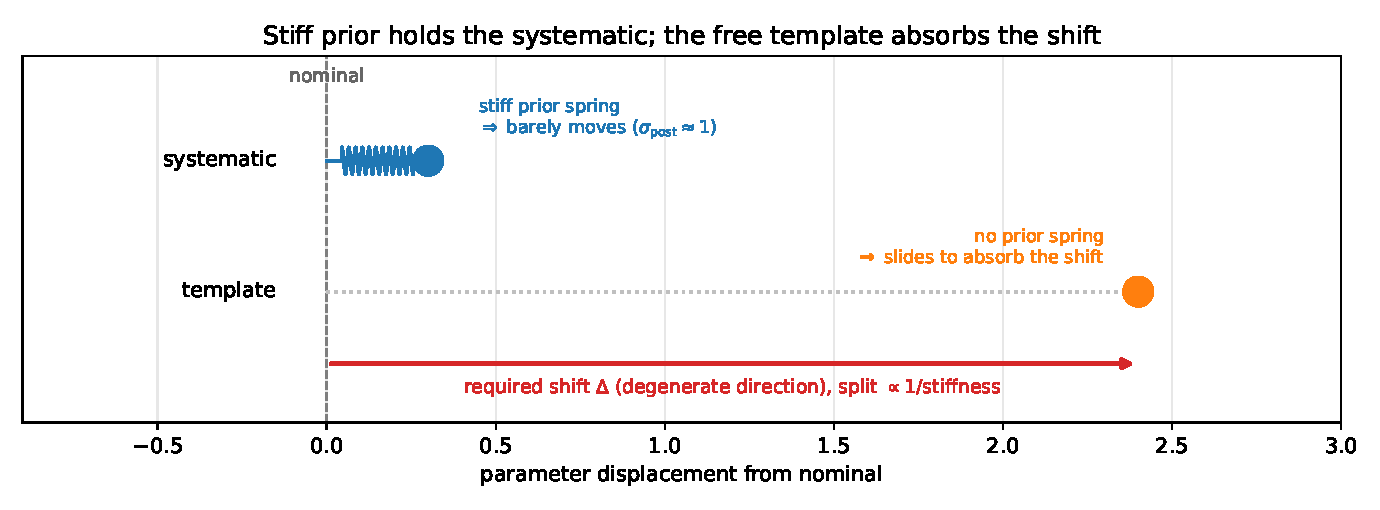
\includegraphics[width=\textwidth]{fig_xsec_spring.pdf}
  \caption{Spring picture of the degeneracy. The prior attaches each systematic
    to its nominal value with a stiff spring (stiffness $2/\sigma_{\rm prior}^2$,
    plus a data spring that grows with the event count); the free template
    parameter has no prior spring. A shift along the degenerate direction is
    shared between the beads in inverse proportion to their stiffness, so the
    free template slides to absorb it while the systematic stays near its prior.
    Low event counts weaken the data spring, pinning the systematic even harder.}
  \label{fig:spring}
\end{figure}

Reading the post-fit
covariance in normalized fit space confirms it: in the \code{all} fit the
flux-beamline and detector sets sit at $\sigma\approx0.998$ and $0.991$
(prior~$=1$), essentially unconstrained, while the templates inflate to
$\sigma\approx1.6$--$2.1$.

\subsection{Why the distribution is precise but the cross section is not}

The distribution is the \emph{product} the data constrains; the cross section is
\emph{one factor} of that product. Isolating the factor means dividing out the
systematic, which is known only to its prior:
\begin{equation}
  \sigma_i \;\propto\; \frac{N_i}{\Phi\,\epsilon_i}
  \quad\Longrightarrow\quad
  \Big(\tfrac{\delta\sigma_i}{\sigma_i}\Big)^2
  \approx \underbrace{\Big(\tfrac{\delta N_i}{N_i}\Big)^2_{\!\text{stat}}}_{\text{distribution}}
  + \Big(\tfrac{\delta\Phi}{\Phi}\Big)^2_{\!\text{prior}}
  + \Big(\tfrac{\delta\epsilon_i}{\epsilon_i}\Big)^2_{\!\text{prior}} + \dots
\end{equation}
The distribution carries only the first term; the cross section carries all of
them. By analogy (Fig.~\ref{fig:rectangle}): measuring the area of a rectangle to
$1\%$ says little about its length if the width is known only to $15\%$---the
length (cross section) inherits the width's (systematic's) prior, not the area's
(distribution's) precision.

\begin{figure}[h]
  \centering
  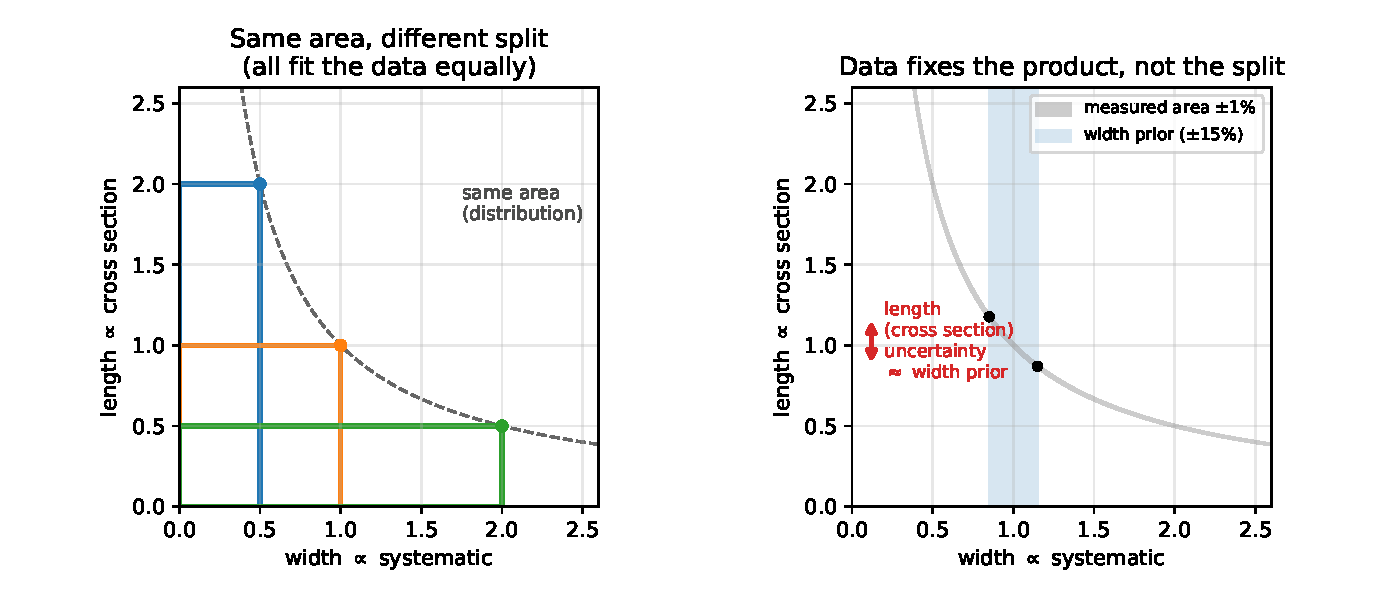
\includegraphics[width=\textwidth]{fig_xsec_rectangle.pdf}
  \caption{Rectangle picture. Left: rectangles of equal area have their corners
    on the hyperbola $\ell = A/w$; the data fixes the area (the distribution) but
    not the split into length ($\propto$ cross section) and width ($\propto$
    systematic). Right: the area is measured tightly (a $\pm1\%$ band), but a
    wide prior on the width ($\pm15\%$) leaves the length uncertain by about the
    width's prior, not the area's precision---the distribution-versus-cross-section
    gap.}
  \label{fig:rectangle}
\end{figure}

In the same true-$E_e$ bins (diagonal binning, \code{all}):

\begin{center}
\begin{tabular}{@{}lc@{}}
\toprule
Quantity (same bins, same fit) & mean fractional unc. \\
\midrule
Post-fit distribution & $8.6\%$ \\
Extracted cross section & $19.1\%$ \\
\bottomrule
\end{tabular}
\end{center}

\subsection{Decomposition of the total uncertainty}

The measurement is \emph{not} statistics-limited. The fiducial signal yield is
$\sim\!450$ events per true-$E_e$ bin ($\sim\!4540$ total), a raw
weighted-Poisson uncertainty of only $\sim\!2.7\%$ per bin. The $23.6\%$ total
(\code{all}, nominal reco binning) is a quadrature sum of several comparable
contributions, isolated as $\sqrt{(\text{variant})^2-(\text{\code{template\_only}})^2}$:

\begin{center}
\begin{tabular}{@{}lcc@{}}
\toprule
Contribution & frac.\ unc. & share of variance \\
\midrule
GENIE                                & $12.2\%$ & $27\%$ \\
Detector                             & $11.6\%$ & $24\%$ \\
Background-diluted fit statistics    & $10.0\%$ & $18\%$ \\
Flux normalization                   & $\phantom{0}9.1\%$ & $15\%$ \\
Flux-beamline                        & $\phantom{0}8.2\%$ & $12\%$ \\
Raw signal Poisson                   & $\phantom{0}2.7\%$ & $\phantom{0}1\%$ \\
\midrule
Total (quadrature)                   & $23.6\%$ & --- \\
\bottomrule
\end{tabular}
\end{center}

Two contributions are flux-related but distinct: the \emph{flux normalization}
(the \code{Constant flux} entry in \code{fitSamples\_TrueEleE.yaml}
\code{normaliseParameterList}, $\sigma=9.13\%$ = hadron production $8.99\%$
$\oplus$ beam focusing $1.62\%$, applied by \code{gundamCalcXsec} to every bin)
and the \emph{flux-beamline} parameter set. No single term dominates, so no one
systematic is a decisive lever. Zeroing the flux normalization
(\code{run\_frac\_uncertainty.sh --zero-flux-norm}) moves the total only from
$23.6\%$ to $21.3\%$, because a $9\%$ term inside a $24\%$ total is only
$\sim\!15\%$ of the variance.

\subsection{The diagonal-response (perfect-resolution) test}

To separate the resolution penalty from the irreducible degeneracy,
\code{run\_frac\_uncertainty.sh --diagonal} bins the fit sample on
\code{true\_leading\_electron\_energy} (\code{binning\_TrueEleE.txt}), so the
``reco'' variable equals the true variable and the response matrix is the
identity.

\begin{itemize}
  \item The total falls only from $23.6\%$ to $19.1\%$, and the stat-only
    (\code{template\_only}) term from $13.6\%$ to $11.3\%$: a $15$--$20\%$
    relative improvement. Resolution is \emph{not} the dominant driver.
  \item The flux-beamline and detector sets go to $\sigma=1.000$ \emph{exactly},
    more degenerate than in reco space. Binning on true energy removes the
    migration dimension, so every systematic acts purely as a per-bin
    rescaling---indistinguishable from the templates.
\end{itemize}

This inverts a natural intuition: resolution/migration is the \emph{only}
feature that gives a systematic a fingerprint distinct from a per-bin template
rescaling, so it is the mechanism by which the fit constrains systematics.
Perfect resolution is the \emph{best} case for constraining them; the diagonal
limit (no migration) is the worst, and makes the degeneracy exact. The gap of
the post-fit $\sigma$ below $1$ in reco space ($0.991$, $0.998$) is exactly the
small part the response matrix makes distinguishable.

With a diagonal response the free templates are exactly degenerate with any
reweighting systematic, so the N$-$1 variants are ill-posed and Migrad diverges
to NaN (the recombination dial is where the NaN first surfaces); the driver
script skips the N$-$1 variants in diagonal mode and still produces the
individual-contribution plots.

\subsection{More statistics does not help}

Only the statistical term scales with POT; the systematic floor is fixed priors.
Projecting the diagonal, flux-norm-removed budget with
stat~$\propto 1/\sqrt{\text{POT}}$:

\begin{center}
\begin{tabular}{@{}lcc@{}}
\toprule
POT & stat term & total xsec unc. \\
\midrule
$2.5\times10^{20}$ (now) & $6.1\%$ & $15.9\%$ \\
$1.0\times10^{21}$       & $3.1\%$ & $14.9\%$ \\
$2.5\times10^{21}$       & $1.9\%$ & $14.7\%$ \\
infinite                 & $0.0\%$ & $14.6\%$ \\
\bottomrule
\end{tabular}
\end{center}

Even infinite statistics reaches only $\sim\!14.6\%$: the measurement is
systematics-limited. In reco space, more statistics marginally tightens the
small non-degenerate part of each systematic ($\sigma<1$); in the diagonal limit
($\sigma=1$) it does nothing.

\subsection{What would reduce it}

\begin{enumerate}
  \item \textbf{Better $E_e$ resolution.} Shrinks the off-diagonal response and
    gives systematics a larger distinguishable fingerprint, letting the fit pull
    them below their priors. Modest, as the diagonal test bounds the gain.
  \item \textbf{An external constraint.} A high-statistics control or sideband
    sample that measures flux and detector directly, so they reach the signal
    fit already narrower than their priors---breaking the template degeneracy
    before it reaches the cross section. This is the only route to the
    few-percent level.
  \item Statistics in the signal sample alone, and removing the flux
    normalization, are \emph{not} effective routes on their own.
\end{enumerate}

%======================================================================
\section{Checklist for a fit}
%======================================================================

\begin{enumerate}
  \item Migrad converged (status 0, small EDM); Hesse matrix accurate and positive
    definite.
  \item Parameters at a bound are either physically sensible (e.g.\ a morph knob
    choosing one model) or understood; for these, \code{llh} rises into the
    allowed region and the uncertainty is quoted as a one-sided interval from a
    scan, not the Hesse error.
  \item No post-fit error exceeds its prior without an explanation.
  \item Post-fit scans have their minimum at the centre, are smooth, and have
    $\Delta\text{llh}=1$ widths consistent with Hesse (allowing for correlations).
  \item Morph knobs use a dial with non-zero slope at nominal (Graph on $[0,1]$, or
    rewritten knots).
  \item In fake-data studies, the knobs that move are the ones expected to absorb
    the injected variation.
\end{enumerate}

\end{document}
